\documentclass[a4paper, 12pt]{book}
\usepackage[utf8]{inputenc}
\usepackage[spanish]{babel} %español
\usepackage{newtxtext}
\usepackage{graphicx}
\usepackage{amsmath}
\usepackage{amsfonts}
\usepackage{amssymb}
\usepackage{graphicx}
\usepackage{float} %Usar [H] en las imagenes y tablas
\usepackage[hidelinks]{hyperref} %Para clikear las pag webs
\usepackage{listings} % color de los bloques de código
\usepackage{minted}
\usepackage[dvipsnames]{xcolor} %color de las letras
% DEFINIENDO COLORES DE LOS CODIGOS
% SQL
\definecolor{codegray}{rgb}{0.5,0.5,0.5}
\definecolor{backcolour}{rgb}{0.95,0.95,0.92}
\lstdefinestyle{estilosql}{
backgroundcolor=\color{backcolour},   
keywordstyle=\color{blue},
numberstyle=\tiny\color{codegray},
basicstyle=\ttfamily\footnotesize,
breakatwhitespace=false,         
breaklines=true,                 
captionpos=b,                    
keepspaces=true,                 
numbers=left,                    
numbersep=5pt,                  
showspaces=false,                
showstringspaces=false,
showtabs=false,                  
}
% Python
\lstdefinestyle{estilopython}{
    backgroundcolor=\color{backcolour},   
    commentstyle=\color{Green},
    keywordstyle=\color{magenta},
    numberstyle=\tiny\color{codegray},
    stringstyle=\color{Orange},
    basicstyle=\ttfamily\footnotesize,
    breakatwhitespace=false,         
    breaklines=true,                 
    captionpos=b,                    
    keepspaces=true,                 
    numbers=left,                    
    numbersep=5pt,                  
    showspaces=false,                
    showstringspaces=false,
    showtabs=false,                  
}
% R es usado con minted

\begin{document}

\author{Gabriel Pinilla}
\title{Resumen comandos para la Ciencia de Datos}

\frontmatter
\maketitle
\tableofcontents %índice
\mainmatter %Número del capítulo sobre el título
% CAPÍTULOS
%
%	CAPITULO SQL
\chapter{SQL en Postgres}
% \textcolor{blue}{}
\lstset{style=estilosql}
%	SECCION
\section{Notas previas...}
\begin{enumerate}
	\item Al finalizar una consulta se debe terminar con ;.
	\item El texto se debe escribir entre comillas simples o dobles, dependiendo del programa a utilizar.
	\item En SQL, el primer caracter de un string inicia con 1 y se escriben entre comillas simples.
	\item Para insertar comentarios se debe usar --
\end{enumerate}
%	SECCION
\section{Comandos básicos}
%	SUBSECCION
\subsection{Estructura básica de una consulta}
La siguiente consulta muestra la estructura básica y el orden que deben seguir los comandos:
\begin{lstlisting}[language=SQL]
SELECT col-sep-por-coma
FROM conj-de-datos.tabla
WHERE condicion
GROUP BY columnas
HAVING condicion
ORDER BY columnas DESC
LIMIT numero;
\end{lstlisting}
Si se requieren todas las columnas de la tabla, se debe agregar un * después del comando \textcolor{blue}{SELECT}.
%	SUBSECCION
\subsection{Where vs Having}
En esta consulta, la cláusula \textcolor{blue}{WHERE} filtra y después el \textcolor{blue}{GROUP BY} agrupa:
\begin{lstlisting}[language=SQL]
SELECT col-sep-por-coma
FROM conj-de-datos.tabla
WHERE condicion
GROUP BY columnas;
\end{lstlisting}
Sin embargo, en la siguiente consulta el \textcolor{blue}{GROUP BY} agrupa y luego el \textcolor{blue}{HAVING} filtra:
\begin{lstlisting}[language=SQL]
SELECT col-sep-por-coma
FROM conj-de-datos.tabla
GROUP BY columnas
HAVING condicion;
\end{lstlisting}
%	SUBSECCION
\subsection{Crear una base de datos}
Para crear una base de datos:
\begin{lstlisting}[language=SQL]
CREATE DATABASE nom-base-de-datos;
\end{lstlisting}
%	SUBSECCION
\subsection{Crear una tabla}
Para crear una tabla:
\begin{lstlisting}[language=SQL]
CREATE TABLE nom-tabla (
    col1 tipo-de-variable,
    col2 tipo-de-variable,
);
\end{lstlisting}
El comando \textcolor{blue}{CREATE TABLE IF NOT EXISTS} crea una tabla si es que dicha tabla no existe en la base de datos.
%	SUBSECCION
\subsection{Insertar datos a una tabla}
Insertar datos a una tabla ya creada:
\begin{lstlisting}[language=SQL]
INSERT INTO tabla (col-sep-por-coma)
VALUES (valores-sep-por-coma);
\end{lstlisting}
%	SUBSECCION
\subsection{Ver todos los datos}
Para ver la tabla completa:
\begin{lstlisting}[language=SQL]
SELECT *
FROM conj-de-datos.tabla;
\end{lstlisting}
%	SECCION
\section{Limpieza, orden y transformación de datos}
%	SUBSECCION
\subsection{Manipulación de filas y columnas}
Para eliminar registros:
\begin{lstlisting}[language=SQL]
DELETE FROM tabla
WHERE nom-col = condicion;
\end{lstlisting}


Agregar una columna:
\begin{lstlisting}[language=SQL]
ALTER TABLE tabla
ADD columna tipo-de-dato;
\end{lstlisting}


Eliminar una datos de una columna:
\begin{lstlisting}[language=SQL]
DELETE conj-de-datos.tabla
WHERE condicion;
\end{lstlisting}


Eliminar una columna:
\begin{lstlisting}[language=SQL]
ALTER TABLE tabla
DROP COLUMN columna;
\end{lstlisting}


Actualizar datos:
\begin{lstlisting}[language=SQL]
UPDATE conj-de-datos.tabla
SET nom-col = valor-a-cambiar
WHERE condicion;
\end{lstlisting}


Eliminar espacios en blanco:
\begin{lstlisting}[language=SQL]
SELECT columna
FROM conj-de-datos.tabla
WHERE
TRIM (columna)=criterio;
\end{lstlisting}


Borrar una base de datos:
\begin{lstlisting}[language=SQL]
DROP DATABASE base-de-datos;
\end{lstlisting}


Borrar una tabla:
\begin{lstlisting}[language=SQL]
DROP TABLE tabla;
\end{lstlisting}


Evitar selecciones duplicadas:
\begin{lstlisting}[language=SQL]
SELECT
DISTINCT (columna)
FROM conj-de-datos.tabla
WHERE condicion;
\end{lstlisting}


Para contar valores distintos:
\begin{lstlisting}[language=SQL]
SELECT COUNT(DISTINCT(col))
FROM conj-de-datos.tabla ;
\end{lstlisting}


¿Cuántas veces aparece cada elemento?
\begin{lstlisting}[language=SQL]
SELECT columna, COUNT (*)
FROM conj-de-datos.tabla
GROUP BY columnas;
\end{lstlisting}
%	SUBSECCION
\subsection{Orden}
Ordenar datos:
\begin{lstlisting}[language=SQL]
SELECT columnas
FROM conj-de-datos.tabla
ORDER BY columna DESC;
\end{lstlisting}
En las consultas SQL, la cláusula \textcolor{blue}{WHERE} filtra los datos según la condición que se le otorgue. Se pueden ordenar los datos en orden ascendente (\textcolor{blue}{ASC}) o descendente (\textcolor{blue}{DESC})
%	SUBSECCION
\subsection{Conversión de tipos}
Para convertir los datos de un tipo a otro se usa la función \textcolor{blue}{CAST}:
\begin{lstlisting}[language=SQL]
SELECT
CAST(columna AS INT) \\
FROM conj-de-datos.tabla; \\
\end{lstlisting}
Los tipos de datos más comunes son:
\begin{enumerate}
\item \textcolor{blue}{SMALLINT}
\item \textcolor{blue}{INTEGER o INT}
\item \textcolor{blue}{BIGINT}
\item \textcolor{blue}{SERIAL}: Número entero que se autoincrementa.
\item \textcolor{blue}{NUMERIC o DECIMAL}
\item \textcolor{blue}{VARCHAR()}: Cadena de caracteres de longitud variable.
\item \textcolor{blue}{TEXT}: Cadena de caracteres de longitud variable que no tiene límite.
\item \textcolor{blue}{DATETIME}
\item \textcolor{blue}{DATE}: Año, mes, día (formato standar).
\item \textcolor{blue}{TIME}: Hora, minuto, segundo.
\item \textcolor{blue}{TIMESTAMP}: Fecha y hora.
\item \textcolor{blue}{BOOLEAN}: TRUE o FALSE.
\end{enumerate}
Si la consulta anterior falla, se puede usar la siguiente consulta:
\begin{lstlisting}[language=SQL]
SELECT
SAFE_CAST(columna AS TIPO-DE-DATO)
FROM conj-de-datos.tabla);
\end{lstlisting}
%	SECCION
\section{Análisis y visualización}
\subsection{Cálculos matemáticos básicos}
Suma (\textcolor{blue}{SUM}) y promedio (\textcolor{blue}{AVG}):
\begin{lstlisting}[language=SQL]
SELECT col, SUM(col2), AVG(col2)
FROM conj-de-datos.tabla
GROUP BY col;
\end{lstlisting}


Mínimo y máximo: Devuelve el valor mínimo de una columna con el nombre de min-columna. Lo mismo para el máximo.
\begin{lstlisting}[language=SQL]
SELECT MIN(columna) AS min-columna,
MAX(col2) AS max-columna
FROM conj-de-datos.tabla;
\end{lstlisting}


Conteo de registros:
\begin{lstlisting}[language=SQL]
SELECT COUNT (*)
FROM conj-de-datos.tabla;
\end{lstlisting}
La consulta anterior contará todos los registros de la tabla. Si se le agrega la cláusula \textcolor{blue}{WHERE} al final, cuenta los registros dependiendo de la condición que tenga.
%	SUBSECCION
\subsection{Número de caracteres de cada fila}
Para que devuelva el número de caracteres:
\begin{lstlisting}[language=SQL]
SELECT
LENGTH(col-para-comprobar-su-largo)
FROM conj-de-datos.tabla;
\end{lstlisting}
También se puede escribir como:
\begin{lstlisting}[language=SQL]
SELECT columna
FROM conj-de-datos.tabla
WHERE
LENGTH(columna)=criterio;
\end{lstlisting}
En algunos programas usan \textcolor{blue}{LEN}. \\
Ejemplo:
\begin{lstlisting}[language=SQL]
SELECT columna1
FROM conj-de-datos.tabla
WHERE
LENGTH(columna1)=5;
\end{lstlisting}
Esta consulta devolverá todos los registros de la columna 1 que tengan 5 caracteres.
%	SUBSECCION
\subsection{Extraer un substring de un string}
\begin{lstlisting}[language=SQL]
SELECT columna
FROM conj-de-datos.tabla
WHERE
SUBSTRS (col, inicio, num-de-letras-a-extraer) + criterio;
\end{lstlisting}
%	SUBSECCION
\subsection{Devolver valores nulos}
\begin{lstlisting}[language=SQL]
SELECT columna
FROM conj-de-datos.tabla
WHERE columna IS NULL;
\end{lstlisting}
%	SUBSECCION
\subsection{Subconsulta}
Es una consulta dentro de otra. Se ejecutan desde la más interna hacia la más externa y van entre paréntesis:
\begin{lstlisting}[language=SQL]
SELECT col-sep-por-coma
FROM conj-de-datos.tabla
WHERE col > (SELECT col-sep-por-coma
             FROM conj-de-datos.tabla);
\end{lstlisting}
%	SUBSECCION
\subsection{Consultas en múltiples tablas}
Para hacer consultas en múltiples tablas, se pued hacer de dos maneras. La primera es usar \textcolor{blue}{SELECT} y \textcolor{blue}{FROM}:
\begin{lstlisting}[language=SQL]
SELECT tabla1.*, tabla2.*
FROM tabla1, tabla 2
WHERE tabla1.columna = tabla2.columna;
\end{lstlisting}
La segunda es usando \textcolor{blue}{JOIN}, los cuales se usan para unir dos tablas bajo la siguiente sintaxis:
\begin{lstlisting}[language=SQL]
SELECT *
FROM conj-de-datos.tabla1
INNER JOIN tabla2
ON tabla1.col= tabla2.col;
\end{lstlisting}
La primera tabla o tabla izquierda siempre irá junto al \textcolor{blue}{FROM}, luego irá la segunda tabla o tabla derecha. Se lee \textit{Tabla 1 hará un cruce con la tabla 2}. \\
Existen 4 formas de cruzar datos:
\begin{enumerate}
\item \textcolor{blue}{INNER JOIN}: Devuelve los registros con valores coincidentes de ambas tablas. No muestra valores nulos.
\begin{figure}[H] 
\centering 
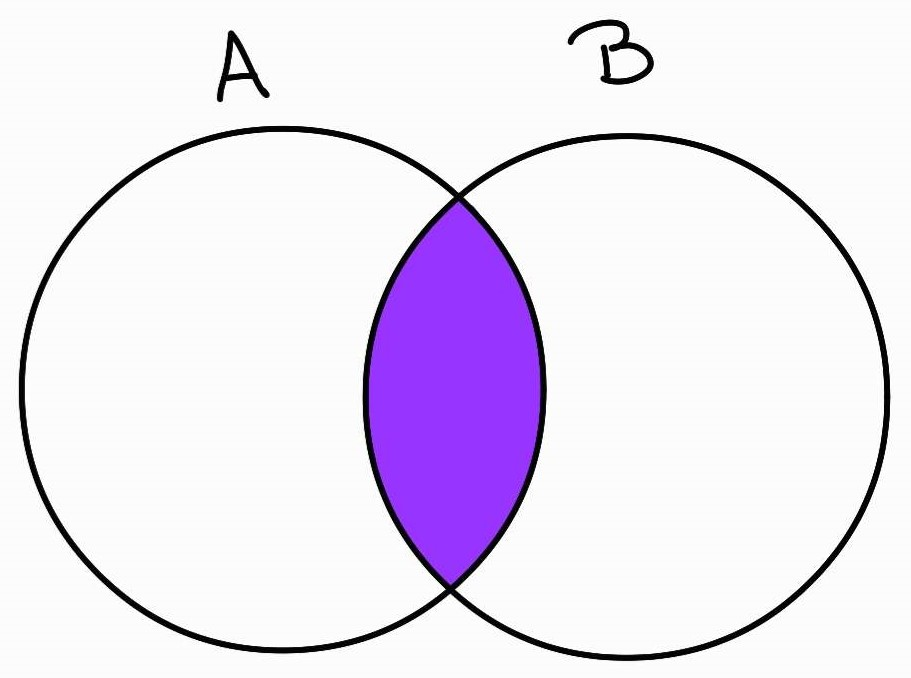
\includegraphics[width=0.4\linewidth]{innerjoin.jpg}
\caption{Diagrama de Venn de INNER JOIN}
\end{figure}
\item \textcolor{blue}{LEFT JOIN}: Devuelve todos los registros de la tabla izquierda y solo los registros coincidentes de la tabla derecha. Tanto en el \textcolor{blue}{LEFT JOIN} como el \textcolor{blue}{RIGHT JOIN} van a mostrar valores nulos. Si hace el cruce con columnas que tienen valores nulos, no cruza esos valores.
\begin{figure}[H] 
\centering 
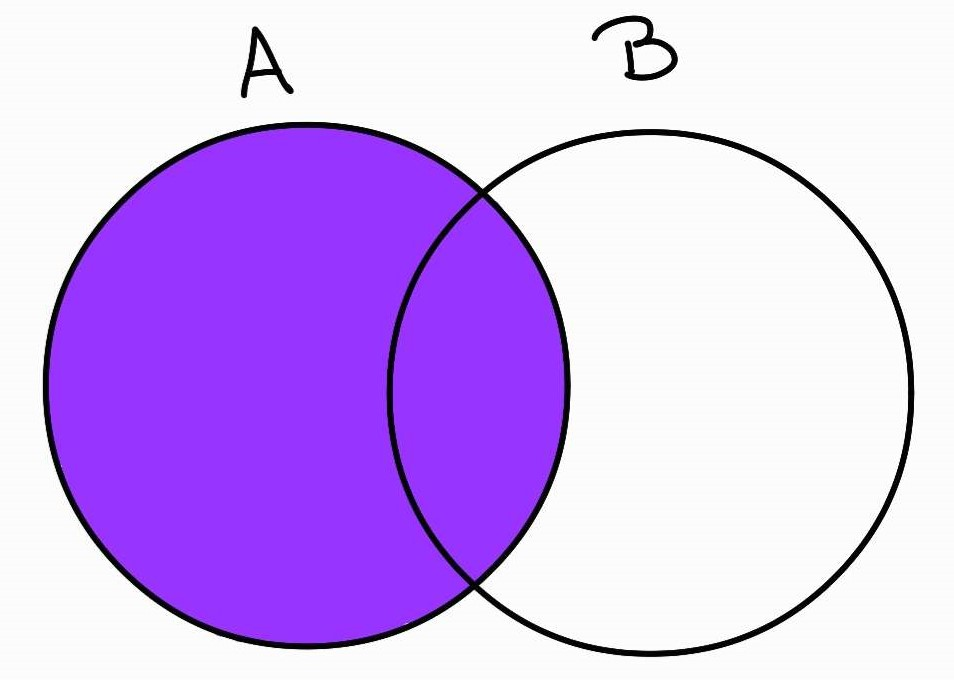
\includegraphics[width=0.4\linewidth]{leftjoin.jpg}
\caption{Diagrama de Venn de LEFT JOIN}
\end{figure}
\item \textcolor{blue}{RIGHT JOIN}: Devuelve todos los registros de la segunda tabla y solo los coincidentes de la primera tabla.
\begin{figure}[H] 
\centering 
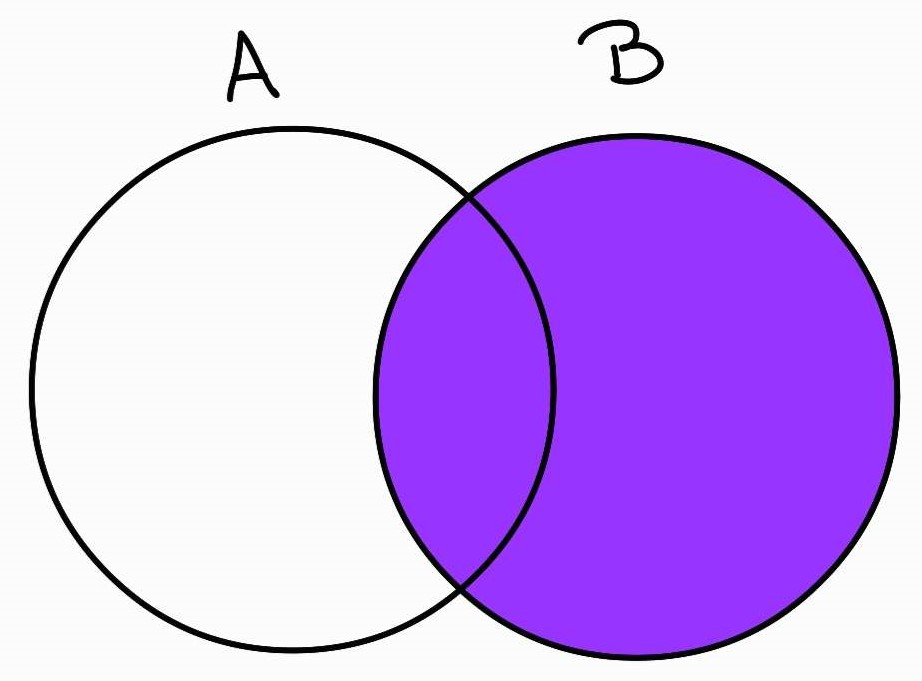
\includegraphics[width=0.4\linewidth]{rightjoin.jpg}
\caption{Diagrama de Venn de RIGHT JOIN}
\end{figure}
\item \textcolor{blue}{FULL JOIN}: Une todos los registros de las dos tablas, sean coincidentes o no.
\begin{figure}[H] 
\centering 
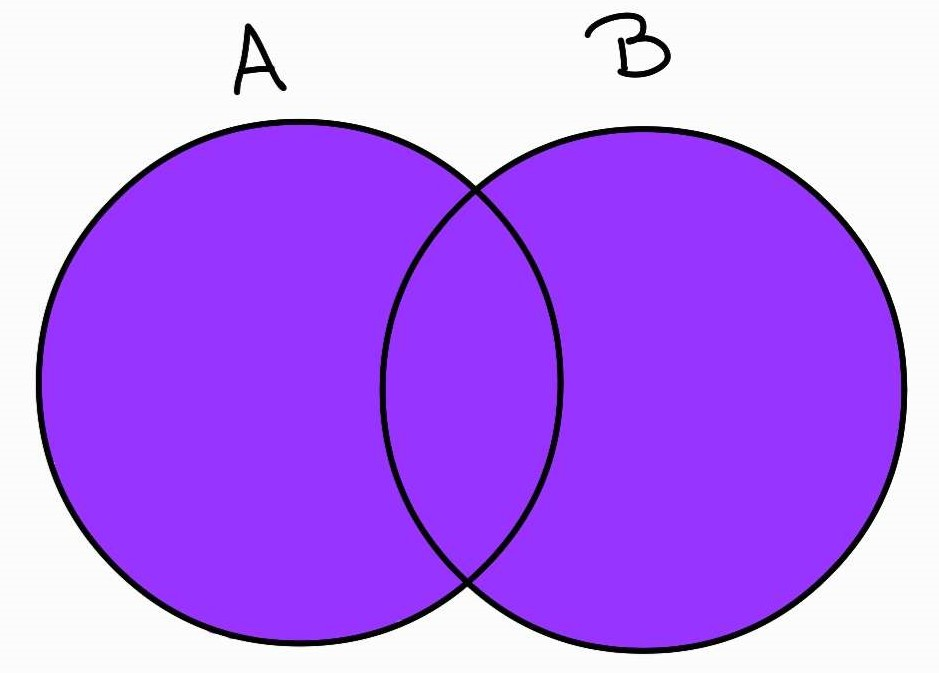
\includegraphics[width=0.4\linewidth]{fulljoin.jpg}
\caption{Diagrama de Venn de FULL JOIN}
\end{figure}
\item \textcolor{blue}{CROSS JOIN}: Combina cada uno de los registros de una tabla con los registros de la otra. No se hace sobre una clave, es decir, no va el \textcolor{blue}{ON}. La tabla resultante tendrá un número de filas igual al producto entre los números de filas de cada tabla, repitiéndose los datos de estas. Debido a esto, ocupa más recursos.
\end{enumerate}
%
%	CAPITULO
\chapter{Terminal Windows}
%	SECCION
\section{Comandos comunes}
\begin{enumerate}
	\item $\setminus$d tabla: muestra información de una tabla y los tipos de datos de cada columna.
	\item $\setminus$c base-de-datos: conectarse a una base de datos.
	\item $\setminus$dt: da una lista de todas las bases de datos.
    \item $\setminus$q: salir de la terminal.
    \item nom-programa version: verifica la versión instalada del programa en el sistema.
    \item clear: limpia la pantalla.
\end{enumerate}
%
%	CAPITULO
\chapter{Excel y Google Sheets}
%\textcolor{Green}{}
%	SECCION
\section{Notas previas...}
\begin{itemize}
\item Algunas funciones de Excel son parecidas a las de Google Sheets.
\item En Google Sheets se usan ; y en Excel ,.
\item Para los rangos se usa C:C, por ejemplo: =MAX(A3:A9).
\end{itemize}
%	SECCION
\section{Comandos básicos}
La sintaxis de una función en Excel y Google Sheets es =NOM-FUNCION(argumento1; argumento2;...), donde los argumentos son los valores que se usan como entrada para la función. \\
Se puede definir la hoja de cálculo con 'nom-hoja'!rango, por ejemplo: =CONTAR.SI('hoja 1'!G:G). En este ejemplo toma toda la columna G de la hoja 1.
%	SECCION
\section{Limpieza, orden y transformación de datos}
%	SUBSECCION
\subsection{Filtrado}
=FILTRAR(rango; fila-o-col = filtro;``"): Devolverá todos los registros del rango, y sin no hay devuelve una cadena vacía (``").
Se pueden crear filtros en Excel: Datos $>$ Filtro.
%	SUBSECCION
\subsection{Orden}
Para ordenar datos en hojas de cálculo, se debe seleccionar Datos $>$ Ordenar. También se puede hacer mediante la función =ORDENAR(). \\
En el siguiente comando, FALSO (o -1 en Excel) indica que el orden es descendiente. Por otro lado, VERDADERO (o 1 en Excel) señala orden ascendente.
=ORDENAR(rango-para-ordenar;segun-columna;FALSO) \\
\\
Usando =ORDENARPOR(): \\
=ORDENARPOR(rango;col-1; FALSO; col-2;VERDADERO)
%	SUBSECCION
\subsection{Quitar duplicados}
Para quitar duplicados en Excel: Datos $>$ Quitar espacios duplicados
%	SUBSECCION
\subsection{Funciones lógicas}
Las funciones lógicas utilizadas en Excel y Google Sheets son:
\begin{itemize}
\item Y(expresion1;expresion2;...)
\item O(expresion1;expresion2;...)
\item NO(valor-logico)
\item =SI(expresion;valor-si-verdadero;valor-si-falso)
\item =SI.ERROR(valor;valor-si-error)
\end{itemize}
%	SUBSECCCION
\subsection{Manipulación de strings}
\begin{enumerate}
\item =ESPACIOS(valores): Elimina espacios del texto.
\item =MAYUSC(celda): Cambia de minúscula a mayúscula.
\item =MINUSC(celda): Cambia de mayúscula a minúscula.
\item =NOMPROPIO(celda): Cambia a nombre propio.
\item =CONCATENAR(): Une dos o más cadenas de texto en una celda.
\item =ENCONTRAR(): Busca una cadena de texto y devuelve su posición.
\item =DERECHA(): Devuelve el número de caracteres iniciando desde la derecha.
\item =IZQUIERDA(): Devuelve el número de caracteres iniciando desde la izquierda.
\item =EXTRAE(): Devuelve un número específico de caracteres de una posición.
\item =LARGO(): Devuelve la longitud de una cadena de texto.
\item =REEMPLAZAR(): Reemplaza una cadena de texto por otra en una celda.
\end{enumerate}
%	SUBSECCION
\subsection{Formatos de fechas}
\begin{enumerate}
\item =HOY(): Devuelve la fecha actual.
\item =AHORA(): Devuelve fecha y hora actual.
\item =FECHA(): Crea una fecha. Ej: =FECHA(2023,6,10).
\item =DIAS360(): Calcula el número de días entre dos fechas en un año de 365 días.
\item =DIAS.LAB(): Calcula el número de días laborales entre dos fechas.
\item =DIAS(): Calcula el número de días entre dos fechas.
\item =MES(): Devuelve el número de mes de una fecha.
\item =AÑO(): Devuelve el año de una fecha.
\item =DIASEM(): Devuelve el número de día de la semana de 1 a 7 para una fecha.
\item =DIAS.LAB.INTL(): Calcula el número de días laborales entre dos fechas usando una definición personalizada de días laborales.
\item =FIN.MES(): Devuelve la fecha del último día del mes antes o después de un número determinado de mesas.
\end{enumerate}
%	SUBSECCION
\subsection{BURSCARV y BURSCARH}
Para relacionar tablas y buscar datos de una tabla a partir de una clave de búsqueda, se usan los comandos BUSCARV y BUSCARH. La principal diferencia entre ellos es que BUSCARV solo realiza la búsqueda en una columna, mientras que BUSCARH lo hace con las filas. \\
Si se escribe FALSO, la coincidencia será exacta. Si se escribe VERDADERO, la coincidencia será cercana. En Excel 1 es verdadero y 0 es falso: \\
=BUSCARV(valor-buscado; rango-de-busqueda; num-para-indicar-col-de-busqueda; FALSO)
%	SUBSECCION
\subsection{Formato de datos}
Se usa la función =CONVERTIR() se usa para transformar un número de un sistema de medición a otro. \\
=CONVERTIR(num-a-convertir;unidad-del-num;unidad-resultado) \\
%	SUBSECCION
\subsection{Formato condicional}
El formato condicional es una herramienta que se utiliza para identificar tendencias resaltándolas con colores. Se le añade una condición para que cambie el aspecto de la celda.


Se puede aplicar el formato condicional de la siguiente forma: \\
Excel: Se debe seleccionar el rango de celdas donde se quiera aplicar el formato $>$ Inicio $>$ Formato condicional $>$ Reglas para resaltar celdas. \\
Google Sheets: Se debe seleccionar el rango de celdas donde se quiera aplicar el formato $>$ Formato $>$ Formato condicional.
%	SECCION
\section{Análisis y visualización}
%	SUBSECCION
\subsection{Cálculos matemáticos básicos}
\begin{enumerate}
\item =SUMA(rango)
\item =PROMEDIO(rango)
\item =MIN(rango)
\item =MAX(rango)
\item =RESIDUO(): Da como resultado el resto cuando al dividir dos números.
\item =CONTAR.SI(rango; ''criterio"): Cuenta el número de celdas que cumplen con un criterio.
\item =SUMAR.SI(rango; ''criterio"): Suma los valores de un rango si cumplen con el criterio.
\item =SUMAPRODUCTO(matriz1;matriz2;...): Multiplica las matrices y muestra el resultado de la suma de esos productos.
\end{enumerate}
%	SUBSECCION
\subsection{Cálculos con múltiples criterios}
\begin{enumerate}
\item =SUMAR.SI.CONJUNTO(rango-suma;rango-criterio1;criterio1;rango-criterio2;criterio2;...)
\item =CONTAR.SI.CONJUNTO(rango-criterio1;criterio1;rango-criterio2;criterio2;...)
\item =MAX.SI.CONJUNTO(rango-max;rango1;criterio1;rango2;criterio2;...)
\end{enumerate}
%	SUBSECCION
\subsection{Tablas dinámicas}
Una tabla dinámica o Pivot Table es una tabla que resume, calcula y analiza datos para observar tendencias entre ellos. \\
Para crear una tabla dinámica tanto en Excel como en Google Sheets, se debe seleccionar Insertar $>$ Tabla dinámica, luego seleccionar los datos preferentemente limpios y con columnas.
%	SUBSECCION
\subsection{Creación de gráficos}
Para crear un gráfico tanto en Excel como en Google Sheets, se debe seleccionar Insertar $>$ Gráfico. Se puede personalizar cambiando los colores, dándole nombre a los ejes y variar el tipo de gráfico.
%	SECCION
\section{Importación de datos}
Si se desea importar datos de otras hojas de cálculo: \\
Excel: Datos$>$Obtener datos$>$ Desde archivo $>$ Desde libro$>$ seleccionar archivo $>$ Importar$>$ seleccionar en el navegador la hoja de trabajo que e quiere importar $>$ Cargar o Transformar datos. \\
Google Sheets: =IMPORTRANGE(), el cual permite especificar un rango de celdas en la otra hoja de cálculo para duplicarlo en la hoja que se esté trabajando.
%	SECCION
\section{Errores}
\begin{itemize}
\item $\#$DIV/0!: Fórmula que intenta dividir por cero un valor en una celda o por una celda vacía. Se soluciona con: =SI.ERROR(valor; valor-si-hay-error).
\item $\#$ERROR!: Error que solo devuelve Google Sheets. Señala que la fórmula no se puede interpretar tal como se ingresa, es decir, hay un error en la fórmula.
\item $\#$N/A: Indica que la hoja de cálculo no puede encontrar los datos de la fórmula. Ocurren generalmente cuando se usa la función =BUSCARV().
\item $\#$NAME? o $\#$NOMBRE?: ocurre cuando el nombre de una fórmula no se reconoce.
\item $\#$NUM!: Señala que el cálculo de una fórmula no se puede realizar según lo especificado por los datos, como por ejemplo una fecha negativa.
\item $\#$VALUE!: Señala un problema con la fórmula o con las celdas con las que hace referencia.
\item $\#$REF!: Aparece cuando las celdas de una fórmula se han eliminado.
\end{itemize}
%
%	CAPITULO
\chapter{Python}
% \texttt{\textcolor{magenta}{}}
\lstset{style=estilopython}
%	SECCION
\section{Notas previas...}
\begin{enumerate}
\item Python es un lenguaje de programación orientado a objetos de alto nivel.
\item Los tipos de datos en Python son int (números enteros), float (decimales), string (cadenas de texto) y booleanos.
\item Los strings se escriben entre comillas simples o dobles.
\item Los comentarios se hacen con el numeral ($\#$). Los comentarios que contengan más de una línea se hacen en un bloque de tres comillas simples:
\begin{lstlisting}[language=Python]
	# Esto es un comentario
	
	'''
	Esto
	es un
	comentario
	'''
\end{lstlisting}
\end{enumerate}

%	SECCION
\section{Librerías}
En ciencia de datos, las librerías más usadas son NumPy, Matplotlib y Pandas.
%	SUBSECCION
\subsection{Importación de datos}
Para importar las librerías, se utiliza el comando \texttt{\textcolor{magenta}{import}} y, usualmente, se le asigna un alias:
\begin{lstlisting}[language=Python]
	import libreria as alias
\end{lstlisting}
Si se quiere importar solo una función de una librería:
\begin{lstlisting}[language=Python]
	from libreria import funcion as alias
\end{lstlisting}
Ejemplo:
\begin{lstlisting}[language=Python]
	# Funcion que genera un numero aleatorio entre 0 y 10
	import random
	num = random.randit(0, 10)
	print('El numero es ', num)
\end{lstlisting}


En Google Colaboratory, se importan los datos de drive con Pandas:
\begin{lstlisting}[language=Python]
	from google.colab import drive
	drive.mount('/content/drive')
\end{lstlisting}
Luego, ir a Archivos $>$ Drive $>$ Copiar ruta de acceso. Se debe importar la librería Pandas con un alias:
\begin{lstlisting}[language=Python]
	import pandas as pd
\end{lstlisting}
Finalmente, para leer un archivo en formato csv:
\begin{lstlisting}[language=Python]
	nom-ds = pd.read\csv('ruta-del-archivo.csv')
\end{lstlisting}

%	SECCION
\section{Manipulación de datos}
%	SUBSECCION
\subsection{Strings}
Los strings son cadenas de textos que contienen una secuencia de caracteres, como palabras. Se definen usando comillas simples o dobles y se pueden realizar operaciones con ellas.

Para interactuar con el usuario, se usan los comandos \texttt{\textcolor{magenta}{print}} y \texttt{\textcolor{magenta}{input}}. El primero imprime un mensaje en pantalla, mientras que el segundo permite que el usuario ingrese datos.
\begin{lstlisting}[language=Python]
	# Imprimir texto en pantalla
	print('Hola mundo')
	
	# Toma informacion y la puede guardar en una variable
	nombre=input('Cual es tu nombre?')
	
	# Sustituir variables en un string
	print(f'Tu nombre es: {nombre}')
	
	# Concatenacion
	print('hola' + ' '+ 'mundo')
	# salida: hola mundo
	
	# Repeticion
	print('Ja' * 4)
	# salida: JaJaJaJa
\end{lstlisting}


Para transformar un número a string:
\begin{lstlisting}[language=Python]
	str(15)
	# salida: 15
	
	print('Quiero ' + str(15) + ' panes')
\end{lstlisting}
Y de un string a número:
\begin{lstlisting}[language=Python]
	edad = int(input('Cual es tu edad?'))
\end{lstlisting}

Operaciones con strings:
\begin{lstlisting}[language=Python]
	texto = 'Hola a todos'
	# 1. lower(): convierte los caracteres a minusculas
	texto_1 = texto.lower()
	print(texto_1)
	# salida: hola a todos
	
	# 2. upper(): convierte los caracteres a mayusculas
	texto_2 = texto.upper()
	print(texto_2)
	# salida: HOLA A TODOS
	
	# 3. replace(sub, new_sub): reemplaza texto por uno nuevo
	texto_3 = texto.replace('todos','Marta')
	print(texto_3)
	# salida: Hola a Marta
	
	# 4. split(sep): divide una cadena en una lista con un separador
	textonuevo = 'Hola,Josesa'
	lista = textonuevo.split(',')
	print(lista)
	# salida: ['Hola', 'Josefa']
	
	# 5. strip(): elimina los espacios en blanco al inicio y final de una cadena
	otrotexto = '	Hola	'
	texto_4 = otrotexto.strip()
	print(texto_4)
	# salida: Hola
\end{lstlisting}

%	SUBSECCION
\subsection{Estructuras de datos}
Listas o arreglos: son secuencias de elementos ordenados por un índice, empezando por el 0.
\begin{lstlisting}[language=Python]
	# Crear una lista
	lista_1 = ['elemento0', 'elemento1', 'elemento2']
	print(lista_1) # Imprime la lista
	
	# Para acceder a los elementos de la lista:
	print(lista_1[0])
	# salida: elemento0
	
	print(lista_1[2]) # o print(lista_1[-1])
	# salida: elemento2
	
	# Para agregar un elemento al final de la lista
	lista_1.append('elemento3')
	print(lista_1)
	# salida: ['elemento0', 'elemento1', 'elemento2', 'elemento3']
	
	# Para obtener la longitud
	longitud = len(lista_1)
	print(longitud)
	# salida: 4
\end{lstlisting}

Diccionarios: es una colección de par clave-valor. Su sintaxis es $\{clave: valor\}$:
\begin{lstlisting}[language=Python]
	diccionario_1={'nombre':'Marcelo',
		'apellido':'Soto',
		'ciudad':'Santiago',
		'edad':38,
		'profesion':'Presidente'}
	
	# Imprimir un valor
	print({diccionario_1['profesion']})
	# salida: Presidente
	
	# Agregar un nuevo par clave-valor
	diccionario_1['estado civil'] = 'Soltero'
\end{lstlisting}

Tuplas: las tupla no se pueden modificar después de haber sido creada.
\begin{lstlisting}[language=Python]
	tupla_1=('elemento0', 'elemento1', 'elemento3')
	
	# Para que devuelva 'elemento0'
	tupla_1[0]
\end{lstlisting}

Set: no permite tener elementos repetidos. Guardará solo los datos que no se repiten.
\begin{lstlisting}[language=Python]
	set_1 = {'banana', 'manzana', 'pera'}
\end{lstlisting}
%	SUBSECCION
\subsection{NumPy Arrays}
NumPy es una librería de Python conocida por los NumPy Arrays o ndarray, una estructura de datos que puede ser de una dimensión (vector), dos dimensiones (matriz), tres (cubo) o más.

Por lo general, se importa con el alias np: \mint{Python}|import numpy as np| Una vez que se importa la librería, 
%	SUBSECCION
\subsection{Tipos de datos de Pandas}
Pandas es una librería la cual permite manipular y analizar estructuras de datos. Se basa en NumPy y proporciona los siguientes tipos de datos:
\begin{enumerate}
	\item Series: Estructuras de una dimensión.
	\item DataFrame: Estructura de dos dimensiones.
	\item Panel: Estructura de tres dimensiones.
\end{enumerate}





%	SUBSECCION
\subsection{Filtrado}

%	SUBSECCION
\subsection{Orden}







% -----------------------------------------------------------

Para mostrar n número de filas del conjunto de datos:
\begin{lstlisting}[language=Python]
nom-ds.head(n)
\end{lstlisting}

Nombres de las columnas del conjunto de datos:
\begin{lstlisting}[language=Python]
nom-ds.columns
\end{lstlisting}

Renombrar columnas, primero se crea un diccionario y luego se utiliza el comando \texttt{\textcolor{magenta}{rename}}:
\begin{lstlisting}[language=Python]
columnas= {'nom-col-1':'nom-col-nueva-1',...}
nom-ds=nom-ds.rename(columns=columnas)
\end{lstlisting}

Para visualizar una muestra del dataset:
\begin{lstlisting}[language=Python]
nom-ds.sample(num-de-registros)
\end{lstlisting}

Información del dataset:
\begin{lstlisting}[language=Python]
nom-ds.info()
\end{lstlisting}

Localizar índice:
\begin{lstlisting}[language=Python]
nom-ds.iloc[indice]
\end{lstlisting}

%	SECCION
\section{Análisis y visualización}
%	SUBSECCION
\subsection{Cálculos matemáticos}
Dimensión del conjunto de datos:
\begin{lstlisting}[language=Python]
nom-ds.shape
\end{lstlisting}

%
%	CAPITULO
\chapter{R}
% \texttt{\textcolor{red}{}}
%	SECCION
\section{Notas previas...}
\begin{enumerate}
\item 
\end{enumerate}
%	SECCION
\section{Paquetes}
Los paquetes en R incluyen funciones, documentación sobre estas mismas, muestras de conjuntos de datos y pruebas para verificar el código. R incluye un conjunto de paquetes denominados Base R. \\
Existe una colección de paquetes llamado Tidyverse que contiene los siguientes paquetes:
\begin{enumerate}
\item ggplot2: se usa para visualizar datos y crear visualizaciones.
\item tidyr: se usa para la limpieza de datos.
\item readr: se usa para importar datos.
\item dplyr: ofrece funciones que ayudan a la manipulación de datos.
\end{enumerate}


Otros paquetes:
\begin{enumerate}
\item here
\item skimr: facilita el resumen de los datos.
\item janitor
\end{enumerate}

Para ver los paquetes instalados:
\begin{minted}{R}
installed.packages()
\end{minted}


Para cargar paquetes:
\begin{minted}{R}
library(paquete)
\end{minted}
%	SECCION
\section{Limpieza}
%	SUBSECCION
\subsection{Resúmenes de datos}
Funciones para obtener resúmenes de los marcos de datos:
\begin{minted}{R}
#Muestra el tipo de datos
str(df)
#Devuelve el min, max, media, mediana, 1er y 3r cuartil. skimr
summary(df)
# skimr
skim_without_charts(df)
# Skimr
skim(df)
# Devuelve el numero de filas y columnas.
glimpse(df)
# Muestra solo las primeras seis filas.
head(df)
\end{minted}
%	SECCION
\section{Orden}
\begin{minted}{R}
# Se usa para elegir qué variable se quiere ordenar.
arrange()
# Para ordenar de forma descendente.
arrange(-)
# Agrupa.
group_by()
# Filtra los datos.
filter()
# Excluye valores NA.
drop_na()
\end{minted}
%	SECCION
\section{Transformación de datos}
\begin{minted}[breaklines, breakanywhere]{R}
# Divide datos en columnas separadas.
separate(df,columna-a-separar, into=c('nom-col-nueva', 'nom-col-nueva-2'), sep= 'tipo-de-separador')
# Permite fusionar columnas entre sí.
unite(df, 'nom-col', col-a-combinar, col-a-combinar-2, sep='separador')
# Se puede usar para añadir columnas con cálculos.
mutate()
\end{minted}
%	SECCION
\section{Cálculos matemáticos}
\begin{minted}{R}
# Media aritmética.
mean()
# Valor máximo.
max()
# Desviación estándar.
sd()
# Correlación.
cor(x=var-x, y=var-y, method='pearson o kendall o spearman')
\end{minted}
%	SECCION
\section{Visualización}
Se utiliza la función ggplot para crear gráficas:
\begin{minted}[breaklines, breakanywhere]{R}
ggplot((data=df) + geom_función(mapping=aes(x=var-x, y=var-y, color=var1, shape=var2, size=var3, alpha=var4))), (color= color-para-todos-los-puntos) + labs() + annotate(text)
\end{minted}


Conceptos de la función ggplot:
\begin{minted}[breaklines, breakanywhere]{R}
# Se inicia un diagrama y se le pueden agregar capas con +.
ggplot()
# Dataset.
data
# Usa puntos para crear diagramas (figura geométrica).
geom_función()
# Define cómo se aplican las variables a las propiedades visuales.
mapping # Va junto a la función aes()
# Especifica qué variables aplicar a los ejes x e y, como el color (color),
# color de relleno (fill), forma de puntos (shape), tipo de línea (linetype)
# y tamaño (size).
aes()
# Grado de transparencia del color.
alpha()
# Se pueden introducir etiquetas como title="", subtitle="", caption="".
labs
# Se utiliza para agregar texto dentro de la cuadrícula.
anotate(text)
# Más información en https://ggplot2.tidyverse.org/reference/annotate.html
\end{minted}


Funciones geom:
\begin{minted}{R}
# Crea diagramas de dispersion.
geom_point()
# Crea graficos de barra.
geom_bar()
# Gráfico de líneas.
geom_line()
# Suavizado. Crea una línea de tendencia.
geom_smooth()
# Crea un histograma.
geom_histogram()
# Crea un diagrama de dispersión y agrega una pequeña cantidad de ruido
#  aleatorio para lidiar con la superposición de puntos.
geom_jitter()
\end{minted}
Cuando se usa la función geom$\_$bar, R cuenta automáticamente cuantas veces aparece cada valor x en los datos y muestra los recuentos en el eje y. Por esta razón, se puede poner en el código solo el eje x. Se puede usar fill para llenar de color las barras. \\
En el caso de geom$\_$histogram, los argumentos de esta funcion son bins=numero, el cual hace referencia al numero de intervalos y binwidth=numero es la amplitud de los intervalos.
%	SUBSECCION
\subsection{Suavizado}
El suavizado permite detectar una tendencia de datos aun cuando no se pueda notar con facilidad una tendencia en los puntos de datos graficados. En ggplot2, suma una línea de suavizado como otra capa en un diagrama. Ayuda a que los diagramas sean más legibles.
\begin{enumerate}
\item El suavizado LOESS es óptimo para suavizar diagramas con menos de 1000 puntos.
\begin{minted}[breaklines, breakanywhere]{R}
ggplot(data, aes(x=, y=))+ geom_point() + geom_smooth(method=”loess”)
\end{minted}
\item El suavizado GAM es útil para suavizar diagramas con un gran numero de puntos.
\begin{minted}[breaklines, breakanywhere]{R}
ggplot(data, aes(x=, y=))+ geom_point() +  geom_smooth(method=”gam”, formula = y ~ s(x))
\end{minted}
\end{enumerate}
%	SUBSECCION
\subsection{Estética y facetas}
Una faceta es una cara o sección de un objeto. Sirve para comparar datos. Permiten mostrar grupos más pequeños, o subconjuntos, de datos.
\begin{minted}{R}
# Facetar el diagrama con una variable.
facet_wrap(~variable)
# Facetar el diagrama con dos variables.
facet_grid(var1~var2)
\end{minted}
%	SUBSECCION
\subsection{Guardar gráficas}
Para guardar una gráfica se puede exportar desde RStudio o usar la función:
\begin{minted}[breaklines, breakanywhere]{R} 
ggsave(“nombre-gráfico.tipo-archivo”, width=ancho, height=largo) # del paquete ggplot2. Ejemplo:
ggsave(“Pingüinos.png”)
\end{minted}
%
%	CAPITULO
\chapter{Markdown}
%
%	CAPITULO
\chapter{Git y GitHub}
%	SECCION
\section{Git}
Se puede hacer correr desde la cmd con el comando \texttt{git}. \\
Lista de comandos:
\begin{itemize}
\item \texttt{git config --global user.name "nom-usuario"}: se configura el nombre de usuario que va entre las comillas. Para configurar el email se debe poner \texttt{git config --global user.email} seguido del email entre comillas.
\item \texttt{git config user.name}: para ver el nombre de usuario. Para ver el email es \texttt{git config user.email}
\end{itemize}
%	SUBSECCION
\subsection{Repositorios}
Para abrir Git en el proyecto, se debe hacer clic derecho Git Bash Here en la carpeta donde se ubica dicho proyecto. Una vez abierto, se puede crear un nuevo repositorio con \texttt{git init} en la rama Master o main.

Con el comando \texttt{git add nom-archivo.extension} se puede enviar archivos al repositorio. Si se quieren subir todos los archivos, se debe usar el comando \texttt{git add .}.

Una vez que se hayan realizado todos los cambios en los archivos, se le puede añadir un comentario con \texttt{git commit -m "Mensaje"} y se suben con \texttt{git push origin nom-rama}.

Si los archivos fueron modificados en GitHub, se pueden bajar al computador con \texttt{git pull}.

Lista de comandos: 
\begin{enumerate}
\item \texttt{git status}: ver el estado del proyecto.
\item \texttt{git commit -m "mensaje"}: se utiliza para tomar una instantánea del proyecto y dejar un mensaje con los cambios realizados en este.
\item \texttt{git log}: para ver todos los mensajes y cambios que han realizado los autores.
\item \texttt{git log --stat}: sirve para visualizar los commits y muestra un pequeño resumen de lo modificado, como la cantidad de líneas e inserciones.
\item \texttt{git log --oneline}: muestra un código que identifica al commit.
\item \texttt{git checkout codigo-commit}: actualiza el archivo para que coincida con el commit señalado en el código-commit. Una vez que se vuelve a un commit anterior, los otros que están en medio se borran. Por esta razón se recomienda trabajar con ramas.
\item \texttt{git rm --cached nom-archivo.extension}: deja de rastrear un archivo sin eliminarlo del directorio de trabajo. Si se quiere hacer con todos los archivos: \texttt{git rm --cached .}.
\item \texttt{git clone direccion-del-repositorio}: clonar un repositorio en el computador.
\item \texttt{touch nom$\_$archivo.extension}: crea un archivo.
\item \texttt{clear}: limpiar la pantalla.
\end{enumerate}
%	SUBSECCION
\subsection{.gitignore}
El archivo .gitignore se crea con fines de que Git ignore ciertos archivos. Para crearlo, se puede hacer mediante la consola de Git con \texttt{touch .gitignore}. Luego de crearlo, se puede abrir con cualquier aplicación y escribir los archivos que se desean ignorar. Se deben escribir los nombres de los proyectos, como mi$\_$proyecto.txt, o se pueden ignorar todas las extensiones, como *.txt.

%	SUBSECCION
\subsection{Ramas}
Una rama en Git es una versión del código de un proyecto, las cuales ayudan a mantener el orden en el control de versiones. El control de versiones es la práctica de gestionar los cambios que se realizan sobre un código. Cuando se habla del estado en el que se encuentra, se refiere a la versión, revisión o edición de este. \\
Cada repositorio en Git comienza con una rama principal predeterminada llamada master. \\
Git almacena una serie de instantáneas al ejecutar el comando commit junto con los metadatos de quién lo haya modificado. \\
Comandos:
\begin{itemize}
\item \texttt{git branch}: devuelve la cantidad de ramas que tiene un proyecto.
\item \texttt{git checkout rama}: cambia de rama.
\item \texttt{git checkout -b nombre-rama}: crear una rama.
\item \texttt{git merge nombre-rama}: unir ramas. El código de nombre-rama se une al de la rama en la que se está trabajando.
\item \texttt{git branch -d nombre-rama}: eliminar una rama solo si la rama se ha fusionado. De lo contrario, usar \texttt{-D} que elimina la rama independientemente de su estado de fusión.
\item \texttt{git branch -d nombre-remoto/nombre-rama}: eliminar una rama remota de VSCode. Generalmente, \texttt{nombre-remoto} es origin.
\end{itemize}

%
%	CAPITULO
\chapter{Tableau Public}
Tableau Public es una plataforma para crear y compartir visualizaciones de datos en línea.

Una visualización de datos es una representación gráfica de los mismos para comunicar información de manera efectiva. Se usa principalmente para identificar patrones que pueden ser difíciles de detectar en una tabla de datos, explorar datos, comunicar información, ayudar a tomar decisiones informadas, hacer seguimiento a procesos, identificar problemas de procesos y más.

%	SECCION
\section{Creación de visualizaciones}
%	SUBSECCION
\subsection{Importación de datos y conexiones}
Para importar datos, se pueden cargar archivos desde el equipo o conectarse con Google Drive. Si se desean agregar más de un archivo, se debe seleccionar el signo + al lado de Conexiones.
\begin{figure}[H] 
	\centering 
	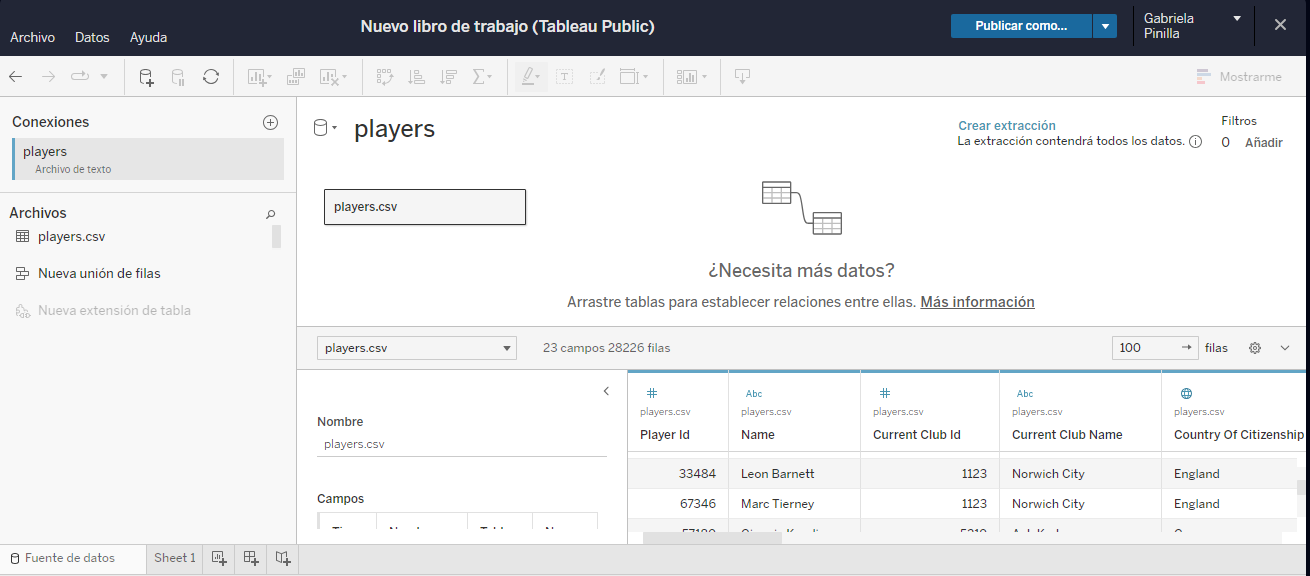
\includegraphics[width=1.0\linewidth]{foto1.png}
	\caption{Fuente de datos}
\end{figure}
En la esquina inferior derecha se muestran los datos en una tabla. Hacia la izquierda en Conexiones, se muestran las fuentes de los datos, los cuales se pueden conectar unos con otros arrastrándolos hacia el panel que dice ¿Necesita más datos?, quedando de la siguiente forma:
\begin{figure}[H] 
	\centering 
	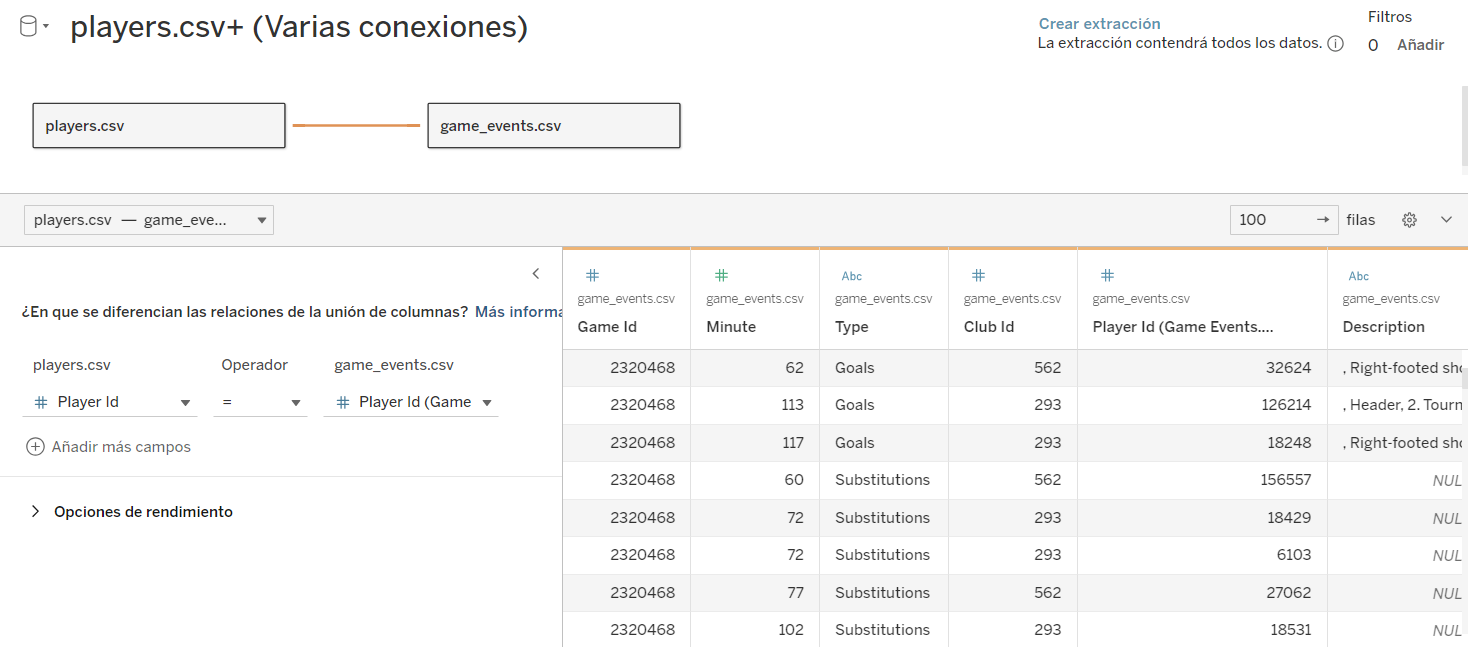
\includegraphics[width=1.0\linewidth]{foto2.png}
	\caption{Campos en común}
\end{figure}
Tableau detecta si hay un campo en común entre ambos archivos csv la cual muestra bajo la conexión de las fuentes.
%	SUBSECCION
\subsection{Campos calculados}
Desde la misma hoja de Fuentes de datos se pueden realizar cálculos en las tablas. Para hacerlo, se debe seleccionar la tabla, luego la flecha de la columna en la que se desea crear un campo calculado, $>$ Crear $>$ Campo calculado...

Se le puede asignar un nombre al campo calculado y escribir la fórmula para calcular los valores del campo seleccionado con los nombres de los campos entre paréntesis de corchetes. Ejemplo: [Campo 1]*5.

En Tableau existen funciones básicas que se pueden utilizar para las fórmulas de los campos calculados:
\begin{enumerate}
	\item CONTAINS: Retorna verdadero si una cadena contiene una subcadena. Ejemplo: CONTAINS("Hola a todos","todos"), devolverá verdadero.
	\item LTRIM: Elimina los espacios en blanco del lado izquierdo de una cadena. Ejemplo: LTRIM("    Hola"), devuelve "Hola".
	\item TRIM: Elimina los espacios en blanco de ambos lados de una cadena. Ejemplo: TRIM("  Hola  "), retorna "Hola"
	\item SPLIT(): Divide un campo según un separador especificado y un token. Ejemplo: SPLIT([Nombre completo], ' ', 2), en el caso de que el nombre sea Juan Soto, devolverá Soto. Si el token es 1, devolverá Juan.
	\item LEN: Devuelve el largo de una cadena de texto. Ejemplo: LEN("Hola a todos"), devuelve 12.
	\item LEFT: Devuelve los primeros caracteres de una cadena según una cantidad especificada. Ejemplo: LEFT("Hola a todos", 4), devuelve "Hola".
	\item RIGHT: Devuelve los caracteres iniciando desde la derecha hacia la izquierda. Ejemplo: RIGHT("Hola a todos", 5), devuelve "todos".
	\item LOWER: Convierte el texto en minúsculas. Ejemplo: LOWER("HOLA"), devuelve hola.
	\item UPPER: Convierte el texto en mayúsculas. Ejemplo: UPPER("hola"), devuelve "HOLA".
	\item MAX: Retorna el valor máximo de una expresión. Ejemplo: MAX([Ventas]), retornará el valor máximo de la columna Ventas.
	\item REPLACE: Reemplaza una subcadena de texo por otra. Ejemplo: REPLACE("Hola a todos", "todos", "todas las mujeres presentes aquí"), devuelve "Hola a todas las mujeres presentes aquí".
	\item COUNT: Muestra la cantidad de filas de un campo. Ejemplo: COUNT([Libros]), devolverá la cantidad de libros.
	\item CEILING: Devuelve el número entero más pequeño mayor o igual que un número especificado. Ejemplo: CEILING(5,13), devuelve 5.
	\item FLOOR: Devuelve el número entero más grande menor o igual que un número especificado. Ejemplo: FLOOR(5,16), devuelve 3.
	\item ROUND: Redondea un número con decimales especificados. Ejemplo: ROUND("5,1634546", 2), devuelve 5,16.
	\item LOG: Devuelve el logaritmo en base e de un número.
	\item DATE: Devuelve la fecha. Ejemplo: DATE(01/05/2023 00:00:00), devuelve 01/05/2023.
	\item DATEDIFF: Devuelve la diferencia entre dos fechas. Ejemplo: DATEDIFF(01/09/2023, 10/09/2023, DAY), devolverá la cantidad de días entre ambas fechas.
	\item DATENAME: Devuelve el nombre de un mes, día de la semana o del año.
	\item DATEPART: Devuelve una parte específica de una fecha. Ejemplo: DATEPART(01/09/2023, YEAR), devolverá 2023.
\end{enumerate}

%	SUBSECCION
\subsection{Conceptos y elementos de Tableau}
Al momento de crear un dashboard, se debe tener en consideración ciertos términos y elementos de la plataforma.

Una hoja de trabajo es un espacio donde se puede construir la visualización de datos. Sus elementos principales son:
\begin{itemize}
	\item Filas y columnas: aquí es donde el usuario puede arrastrar los campos de datos para definir las dimensiones y medidas de la visualización.
	\item Dimensiones y medidas: en el panel de datos se pueden encontrar los datos divididos por una línea donde los de arriba representan las dimensiones y los de abajo las medidas. 
	\begin{itemize}
		\item Las dimensiones son los datos categóricos. Su fin es clasificar la información. Los tipos de dimensiones son: fechas, cadenas de texto, booleanos (verdadero o falso) y rol geográfico. Ejemplo: género, estado civil.
		\item Las medidas son datos de origen cuantitativos que asignan valores a las dimensiones. Los tipos de medidas son: números y rol geográfico (latitud y longitud). Ejemplo: cantidad de habitantes.
	\end{itemize}
	  En este mismo panel, se encuentran datos de color azules, los cuales corresponden a datos discretos. Se tratan como finitos. Por el contrario, los verdes son datos continuos. Se tratan como un intervalo infinito.
	\item Marcas: en la tarjeta de marcas se configura la forma en que las dimensiones y medidas serán representadas. Sus elementos son: Tipo de marca: el cual indica la forma en la que se van a graficar los datos; Color: permite cambiar los colores de la visualización; Tamaño: varía el tamaño de la visualización; Texto: permite definir el texto de la etiqueta a mostrar en la gráfica; Detalle: permite agregar información a las marcas; Descripción emergente: permite que al pasar el mouse por una marca se muestre una descripción emergente con información.
	\begin{figure}[H] 
		\centering 
		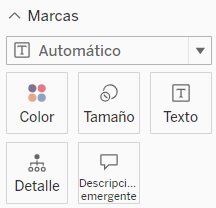
\includegraphics[width=0.3\linewidth]{marcas.png}
		\caption{Tarjeta de marcas}
	\end{figure}
	\item Filtros: aplica filtros al arrastrar los campos a este estante.
	\item Páginas: se pueden arrastrar campos para crear páginas en la visualización.
\end{itemize}

%	SUBSECCION
\subsection{Filtros}
\begin{enumerate}
	\item Filtros de extracción: se usan para limitar el conjunto de datos desde la Fuente de datos. Al aplicarlo, se abrirá una ventana para añadir los filtros que se deseen.
	\begin{figure}[H] 
		\centering 
		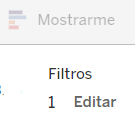
\includegraphics[width=0.2\linewidth]{filtro1.png}
		\caption{Filtro de extracción}
	\end{figure}
	\item Filtros de contexto: se usan para definir un contexto específico en los cálculos. En lugar de aplicar un filtro para el conjunto de datos, crea un subconjunto de datos para hacer cálculos. Para crear un filtro de contexto, se debe arrastrar un campo al estante de filtros en la hoja de trabajo, luego seleccionar la flecha de la cápsula del campo y seleccionar Añadir a contexto.
	\begin{figure}[H] 
		\centering 
		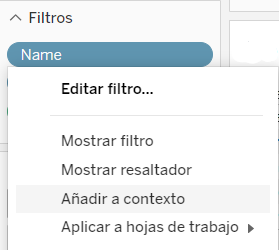
\includegraphics[width=0.3\linewidth]{filtro2.png}
		\caption{Filtro de contexto}
	\end{figure}
	\item Filtro de dimensión: se usan para filtrar datos de dimensiones discretas.
	\begin{figure}[H] 
		\centering 
		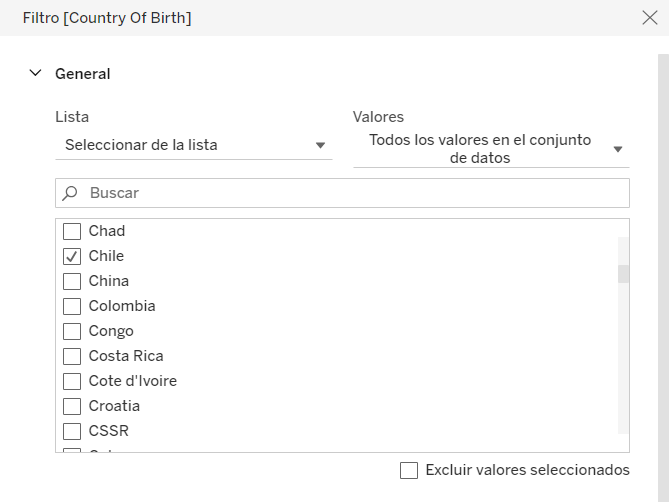
\includegraphics[width=0.6\linewidth]{filtro3.png}
		\caption{Filtro de dimensión}
	\end{figure}
	\item Filtro de medida: se usan para filtrar datos en función de una medida continua.
	\begin{figure}[H] 
		\centering 
		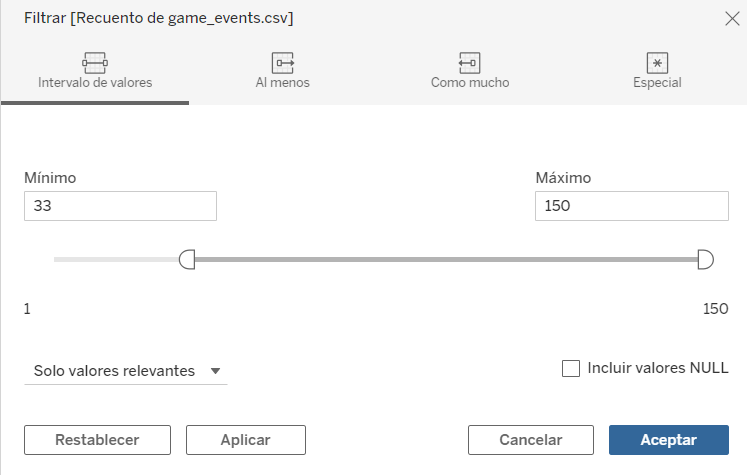
\includegraphics[width=0.5\linewidth]{filtro4.png}
		\caption{Filtro de medida}
	\end{figure}
	\item Filtro en gráfico: se pueden filtrar datos en un gráfico.
\end{enumerate}

%	SECCION
\section{Creación de visualizaciones básicas}
La creación de visualizaciones en Tableau se hace arrastrando las tablas de datos hacia los estantes de filas, columnas, marcas y filtros.

En el siguiente ejemplo se utilizó la base de datos del siguiente enlace de Kaggle \url{Uhttps://www.kaggle.com/datasets/ishikajohari/shazam-global-top-200-per-week?resource=download}, el cual muestra datos del top 200 por semana de Shazam, una aplicación para identificar música y otros desde los dispositivos móviles.

Con la base de datos de la primera semana (Week1 -22-Jul-to-28-Jul-2023.csv), se construyó la siguiente tabla:
\begin{figure}[H] 
	\centering 
	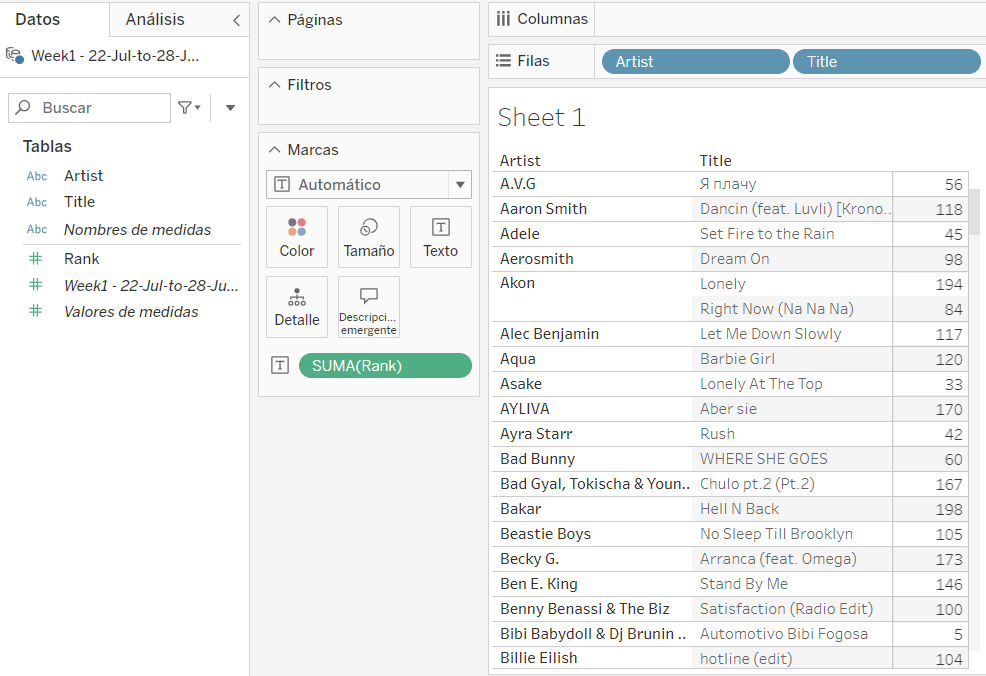
\includegraphics[width=0.9\linewidth]{tabla1.png}
	\caption{Tabla de datos creada en Tableau}
\end{figure}
En el estante de filas se añadieron Artist (dimensión) y Title (dimensión), mientras que Rank (medida) se añadió a Texto en Marcas, mostrando en la tabla el rankin de la canción y al artista a quien le pertenece. Por defecto, Tableau añade una función de agregación, que en el caso del ejemplo es SUMA, sin embargo, como se trata de un rankin, solo corresponde a un número y no a una suma.

En la misma tabla, se pueden ordenar los datos por el rankin, como de mayor a menor, sin embargo, al tener dos dimensiones en las filas no mostrará cuál canción es menos escuchada en el rankin, sino que mostrará un conjunto de canciones con su rankin perteneciente al mismo artista.
\begin{figure}[H] 
	\centering 
	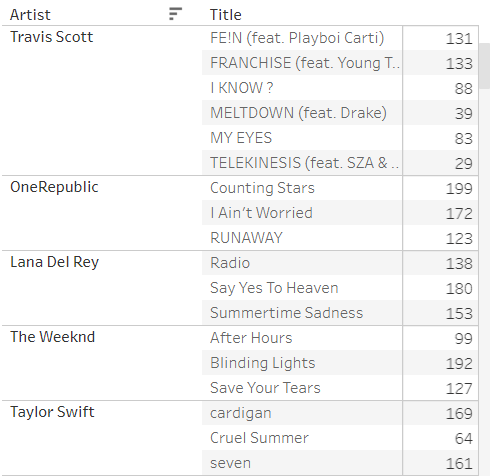
\includegraphics[width=0.5\linewidth]{tabla2.png}
	\caption{Tabla de datos creada en Tableau}
\end{figure}
Para descubrir cuál es la canción menos escuchada, se debe dejar solo una dimensión en filas, como Title, y luego ordenarlas. Si se quiere saber cuál es el artista menos escuchado, se debe hacer lo mismo con la dimensión Artist.
\begin{figure}[H] 
	\centering 
	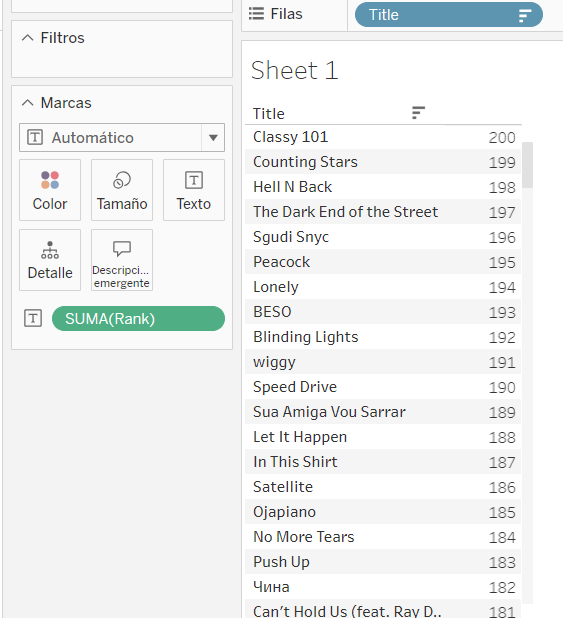
\includegraphics[width=0.7\linewidth]{tabla3.png}
	\caption{Tabla de datos creada en Tableau}
\end{figure}
También, se puede modificar la medida Rank para que cuente la cantidad de canciones con la que los artistas aparecen en el rankin.
\begin{figure}[H] 
	\centering 
	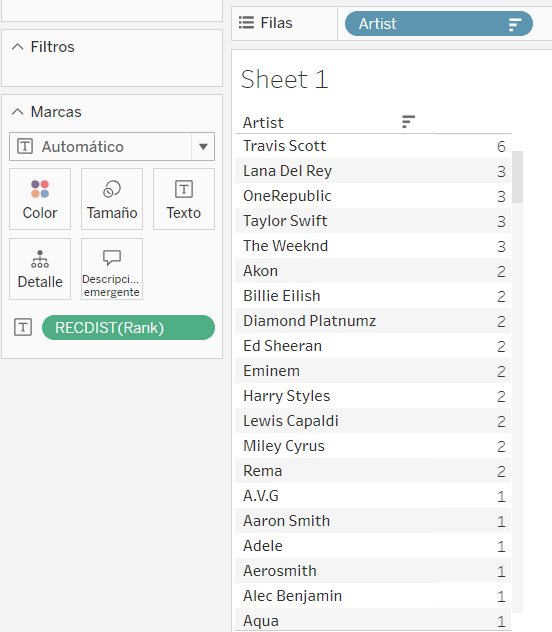
\includegraphics[width=0.7\linewidth]{tabla4.png}
	\caption{Tabla de datos creada en Tableau}
\end{figure}


Para el siguiente ejemplo, se tomó la base de datos mensual de las 50 principales cuentas de redes sociales de
\url{https://www.kaggle.com/datasets/amyrmahdy/monthly-top-50-social-media-accounts-dataset}.

Con al base de datos del top 50 de Youtube (youtube$\_$top$\_$50$\_$2023-07-03), se construyó la siguiente visualización:
\begin{figure}[H] 
	\centering 
	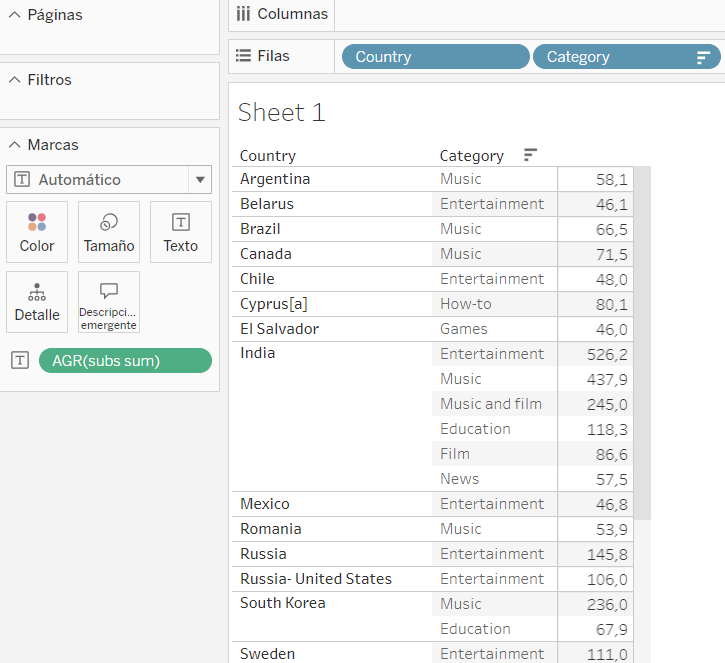
\includegraphics[width=0.7\linewidth]{tabla5.png}
	\caption{Tabla de datos creada en Tableau}
\end{figure}
Esta tabla muestra la categoría (Category) de cada país (Country) ordenado de mayor a menor por la suma de los subscriptores (subs sum) de cada categoría. Esta suma se realizó en el campo calculado de la Fuente de datos con el código SUM([Subscribers (millions)]).

Sin embargo, estos datos también se pueden representar de forma geoespacial por medio de un mapa.
\begin{figure}[H] 
	\centering 
	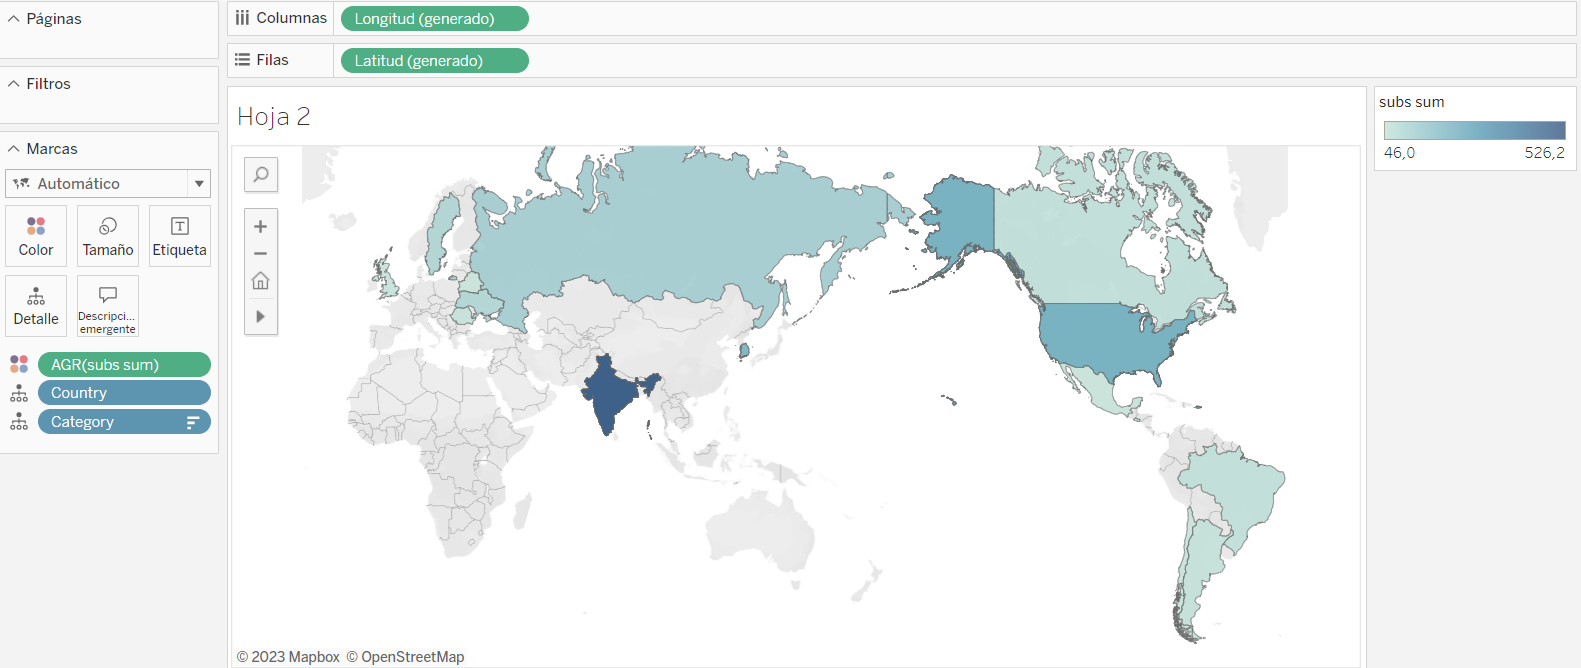
\includegraphics[width=0.9\linewidth]{mapa1.png}
	\caption{}
\end{figure}
Ordenando los subscriptores de forma descendente, se obtiene un mapa que muestra la categoría con más subscriptores en los países, donde el color azul indica un número más alto que el color celeste claro.

Para hacer esto, se agregó la tabla de subscriptores a la marca de Color, de esta forma Tableau puede hacer un mapa de calor indicando qué países tienen una mayor cantidad de subscriptores. La categoría y el país se arrastraron hacia la marca de Detalles, por lo que al pasar el mouse por encima de alguno de estos países mostrará el nombre del país, la categoría y la cantidad de subscriptores. La latitud y longitud en filas y columnas se generó a partir de la tabla Country.

%	SECCION
\section{Diseño y personalización de paneles}
Al graficar, se debe tener en consideración el tipo de datos que presenta la base de datos dado que no todos los gráficos sirven para representar cualquier tipo de datos.

Para elegir un gráfico que va a representar un conjunto de datos, es importante saber qué es lo que se quiere mostrar con la visualización, conocer los tipos de gráficos y saber cuál es la audiencia a quienes se les va a presentar.

A continuación, se presentan algunos tipos de gráficos:
\begin{enumerate}
	\item Gráfico de columnas: Compara categorías usando barras verticales.
	\item Gráfico de barras: Compara categorías usando barras horizontales.
	\item Gráfico circular: Proporciona las categorías en relación al total.
	\item Gráfico de líneas: Muestra las tendencias a lo largo del tiempo usando líneas.
	\item Gráfico de área: Muestra las tendencias a lo largo del tiempo usando un área sombreada bajo la línea.
	\item Gráfico de dispersión: Relaciona dos conjuntos de datos usando puntos.
	\item Gráfico de burbujas: Relaciona dos conjuntos de datos usando burbujas de diferentes tamaños para mostrar la magnitud de un tercer conjunto de datos.
	\item Histograma: Distribuye los datos en un rango continuo.
	\item Gráfico de radar: Expone los datos en un formato circular con categorías que se extienden radialmente.
\end{enumerate}

%	SUBSECCION
\subsection{Funciones de agregación}
Las funciones de agregación son una funciones que operan sobre un conjunto de datos que devuelven un único valor. Se pueden obtener el promedio de un conjunto, máximo, mínimo, recuento o suma.

Las funciones de agregación más comunes en Tableau son:
\begin{itemize}
	\item Promedio
	\item Suma
	\item Promedio o media
	\item Mediana
	\item Recuento: devuelve la cantidad de filas. Ejemplo: Rec(a,a,b,b)=4.
	\item Recuento (distintos): devuelve la cantidad de valores distintos de una columna. Ejemplo: RecDis(a,a,b,b)=2.
	\item Máximo y mínimo
	\item Desviación estándar y desviación estándar poblacional
	\item Varianza y varianza poblacional
\end{itemize}
Para agregar una función de agregación, se debe seleccionar Medida $>$ Suma, Promedio, Mediana...

Por defecto, Tableau agrega la suma para medidas numéricas y el recuento para las no numéricas.
%	SUBSECCION
\subsection{Funciones LOD}
Las funciones LOD (Level of Detail) en Tableau permite realizar cálculos en un nivel de detalle específico en los datos. Son útiles cuando se requiere realizar cálculos que no se pueden lograr con las funciones de agregación.

Tableu tiene tres tipos de funciones LOD:
\begin{enumerate}
	\item FIXED: permite definir un nivel de detalle específico para un cálculo. Ejemplo: Para calcular la suma de ventas por categoría: {FIXED [Categoria] : SUM([Ventas])}.
	\item INCLUDE: permite incluir un nivel de detalle específico a un cálculo sin afectar el nivel de detalle general de la visualización. Ejemplo: Para calcular la suma de ventas por categorías e incluir la ciudad: {INCLUDE [Categoria],[Ciudad] : SUM([Ventas])}.
	\item EXCLUDE: permite excluir un nivel de detalle específico a un cálculo sin afectar el nivel de detalle general de la visualización.
\end{enumerate}

%	SECCION
\section{Dashboards}
Un dashboard consiste en una pantalla que presenta una colección de visualizaciones que resumen información importante.

Uno de los propósitos de un dashboard es monitorear el rendimiento de un a empresa por medio de KPI, presentando la información de forma clara para que el público pueda entenderla.

Un KPI (Key Performance Indicator o Indicador Clave de Rendimiento) es una medida que evalúa el rendimiento de una empresa o proceso con respecto al objetivo empresarial. Los KPI siguen la metodología S.M.A.R.T., un acrónimo que explican las características básicas de un objetivo SMART. Estos deben ser específicos (Specific), medibles (Measurable), alcanzables (Attainable), realistas (Realistic) y con un tiempo límite (Time).

Ejemplos de métricas que se pueden usar para los KPI:
\begin{itemize}
	\item ROI
	\item Número de clientes nuevos
	\item Tasa de satisfacción
	\item Tasa de rotación del personal
	\item Porcentaje de clics en una página web
	\item Cantidad de carritos de compras abandonados
	\item IPC
\end{itemize}
%	SUBSECCION
\subsection{Creación de un dashboard}
Para crear un dashboard, se debe seleccionar el icono de Nuevo dashboard.

Luego, arrastrar las vistas desde la lista de Hojas hacia el dashboard.



\begin{thebibliography}{0}
\bibitem{} \url{https://www.javatpoint.com/postgresql-tutorial} %SQL POSTGRES CODE
\bibitem{} \url{https://git-scm.com/doc} %documentación git
\bibitem{} \url{https://git-scm.com/book/es/v2} %libro en español de git
\bibitem{}  \url{https://help.tableau.com/current/pro/desktop/es-es/dashboards_create.htm}
\bibitem{} \url{https://docs.python.org/es/3/index.html}
% https://bookdown.org/paradinas_iosu/CursoR/ggplot2.html#temas -> ir a la pregunta más popular
% \bibitem{} \url{https://manualdelatex.com/simbolos} SIMBOLOS LATEX
% https://es.overleaf.com/learn/latex/Using_colours_in_LaTeX -> colores latex
\end{thebibliography}
% NOTAS:
% Doble comillas: ``"
% https://es.wikibooks.org/wiki/Manual_de_LaTeX/Listados_de_código/Listados_con_minted



\end{document}